\subsubsection{Foundations of Deep Learning} \label{sec:dl-foundations}

This section explores the fundamental principles of \ac{DL}, with a specific focus on activation functions and backpropagation. Activation functions play a vital role in neural networks by introducing non-linearity and enabling the representation of complex relationships. This section covers the most commonly used activation functions. In addition, this section discusses the backpropagation algorithm, which plays a crucial role in training feedforward neural networks by calculating gradients with respect to network weights for iterative adjustments and optimal model performance. Furthermore, this section explores optimization techniques within deep learning.

\paragraph{Activation Functions} \label{sec:activation}

Activation functions are essential to neural networks, as they introduce non-linearity into the model. Nonlinearity is important because it allows the model to learn complex relationships between inputs and outputs. This section will discuss some of the most commonly used activation functions, including sigmoid, \ac{tanh}, and \ac{ReLU}.

\begin{figure}[ht]
    \centering
    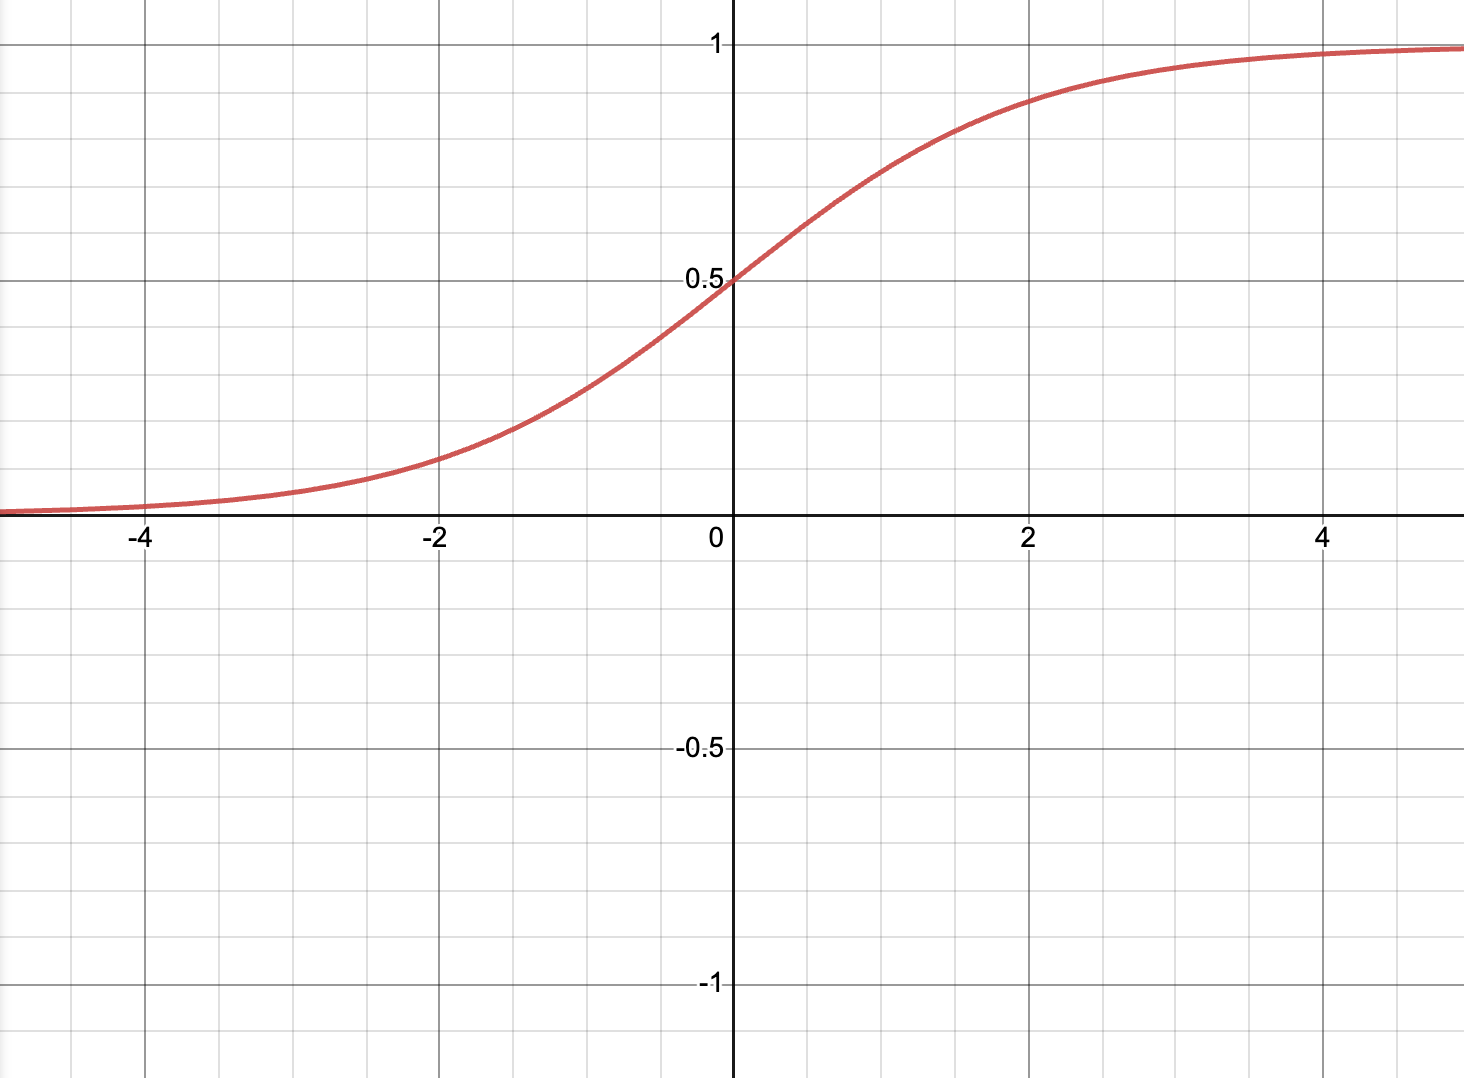
\includegraphics[width=\textwidth/2]{figures/2-sota/activation/sigmoid.png}
    \caption[Sigmoid Activation Function]{One can see that the values that are output are exclusively between 0 and 1 with its value being 0.5 for $x = 0$.}
    \label{fig:sigmoid}
\end{figure}

\label{sec:sigmoid}

The \textbf{sigmoid} activation function is prevalent in neural networks. It is defined as:

\begin{equation}
	\sigma(x) = \frac{1}{1 + e^{-x}}
\end{equation}

where $x$ is the input to the function. The output of the sigmoid function is always between 0 and 1, which makes it useful for binary classification tasks. The sigmoid function is also differentiable, which is essential for backpropagation during training. Figure \ref{fig:sigmoid} visually represents this function.

However, the sigmoid function has a few drawbacks. One issue is that the function's gradient approaches zero as the input becomes very large or very small. This can cause the weights to update very slowly during training, a problem known as the \textit{vanishing gradient} problem. Additionally, the output of the sigmoid function is not zero-centered, which can make optimization more difficult. On the other hand, if the gradients become extremely large, it can cause the weights to update too much in each iteration, leading to the \textit{gradient explosion problem}. This can lead to the model diverging and failing to converge to a good solution. 

\label{sec:tanh}

The \textbf{\acf{tanh}} activation function is similar to the sigmoid function, but its output is between -1 and 1:

\begin{equation}
	\tanh(x) = \frac{e^x - e^{-x}}{e^x + e^{-x}}
\end{equation}

Tanh is differentiable and valuable for binary classification tasks like the sigmoid function. However, it has the same vanishing gradient problem as the sigmoid function. A visual representation can be seen in Figure~\ref{fig:tanh}.

\begin{figure}[ht]
    \centering
    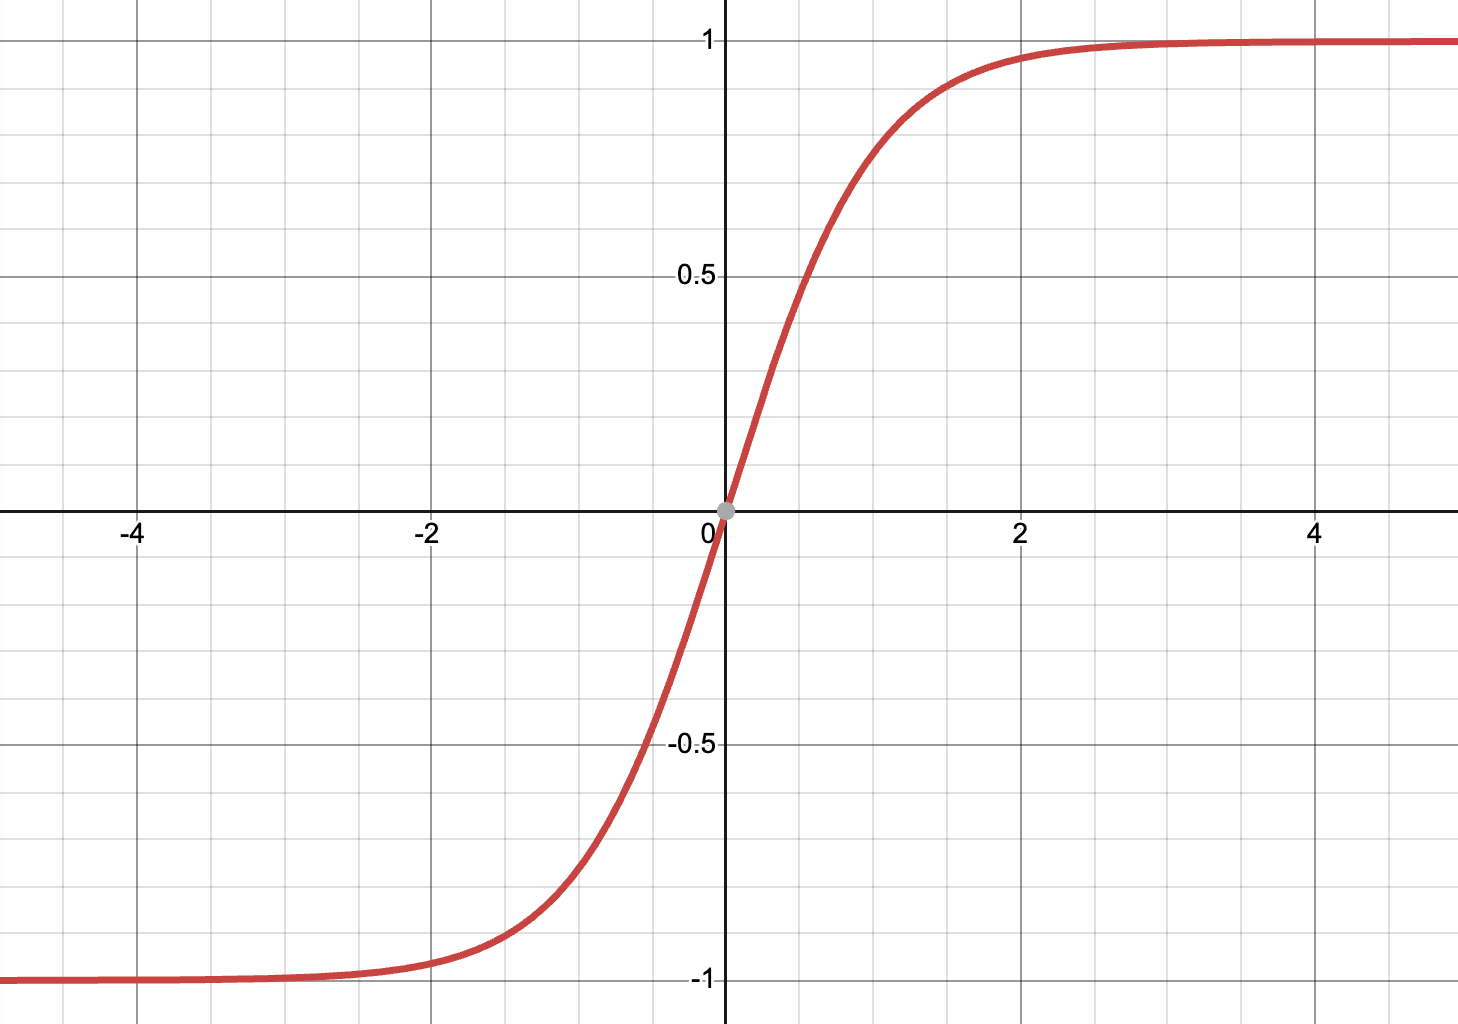
\includegraphics[width=\textwidth/2]{figures/2-sota/activation/tanh.png}
    \caption[Tanh Activation Function]{A very similar function except that its limits are present on -1 and 1}
    \label{fig:tanh}
\end{figure}

\label{sec:relu}

The \textbf{\acf{ReLU}} activation function is a popular choice in \ac{DL}. It is defined as:

\begin{equation}
	\text{ReLU}(x) = \max(0, x)
\end{equation}

The \ac{ReLU} function is also zero-centered, which can make optimization easier. However, this function is not differentiable at $x=0$, which can cause problems during training. Variants of the \ac{ReLU} function have been proposed to address this issue. A visual representation can be seen in Figure \ref{fig:relu}.

\begin{figure}[ht]
    \centering
    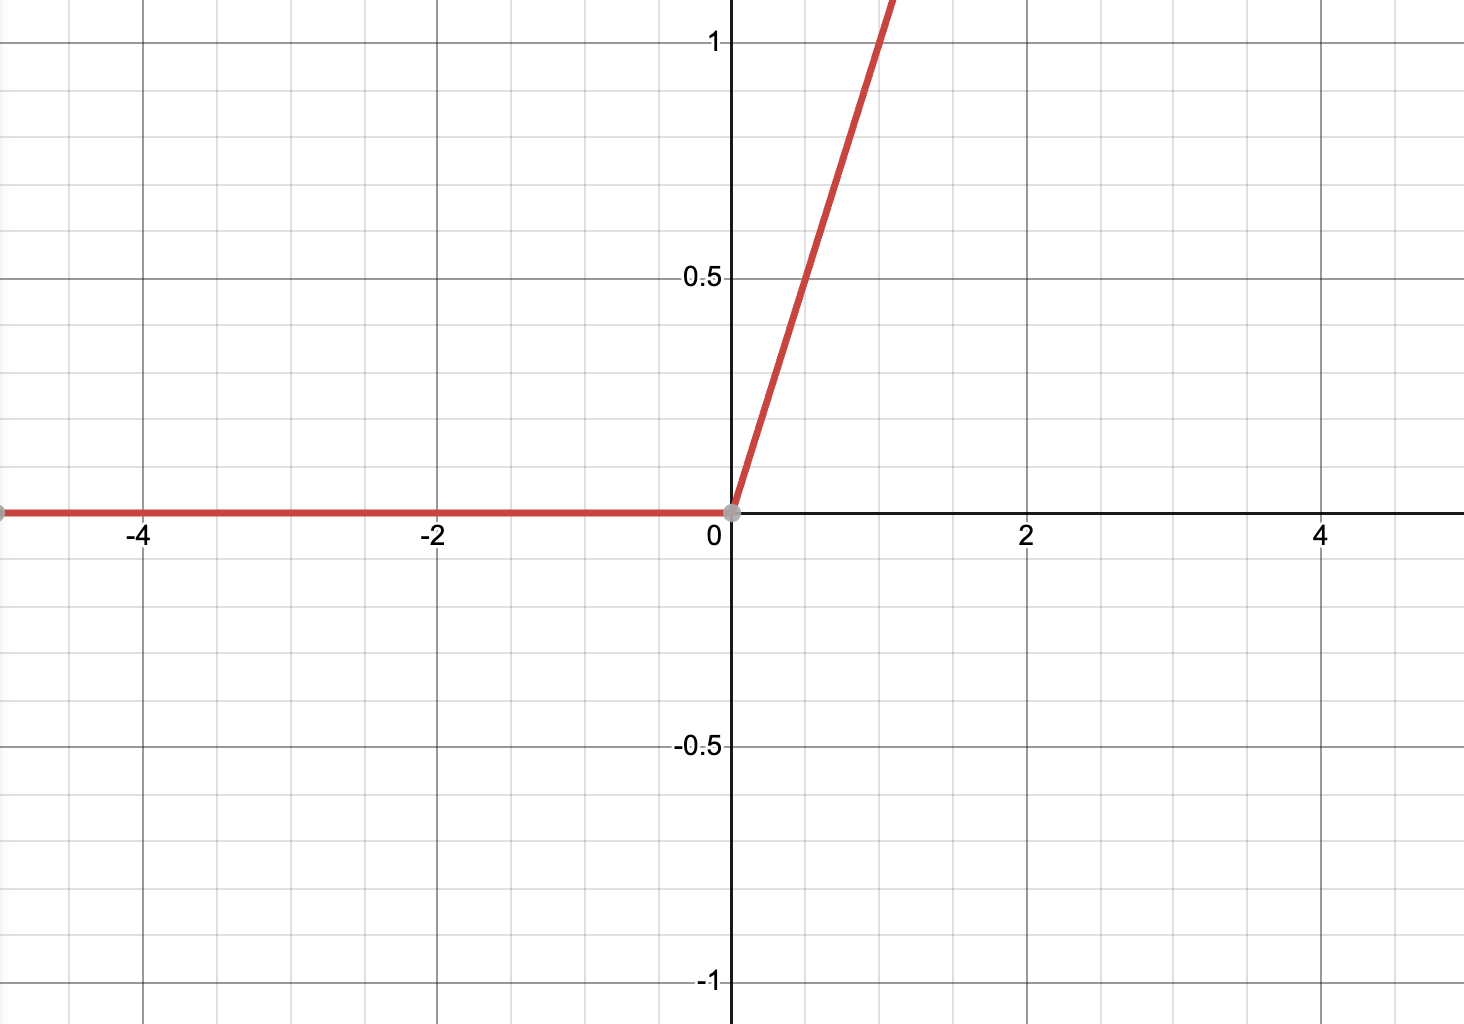
\includegraphics[width=\textwidth/2]{figures/2-sota/activation/relu.png}
    \caption[Relu Activation Function]{Linear for positive values, 0 for negative values.}
    \label{fig:relu}
\end{figure}

The \ac{ReLU} activation has a potential problem known as the \textit{dying ReLU} problem. When a neuron's weights become such that its input is always negative, its gradient will always be zero. In this situation, the neuron will become inactive, or \textit{dead}, and will no longer update during training. This problem can lead to underfitting, as some neurons stop learning and contributing to the model. Variants of \ac{ReLU}, such as \textbf{Leaky \ac{ReLU}}, have been proposed to mitigate the dying \ac{ReLU} problem by assigning a slight non-zero gradient for negative input values.

The Leaky ReLU function is defined as:

\begin{equation}
\text{Leaky ReLU}(x) = \text{max}(a x , x)
\end{equation}

where $a$ is a small positive number such as $0.01$. This non-zero gradient for negative inputs can help prevent neurons from becoming inactive during training. This function can visually be seen in Figure~\ref{fig:leaky-relu}.

\begin{figure}[ht]
    \centering
    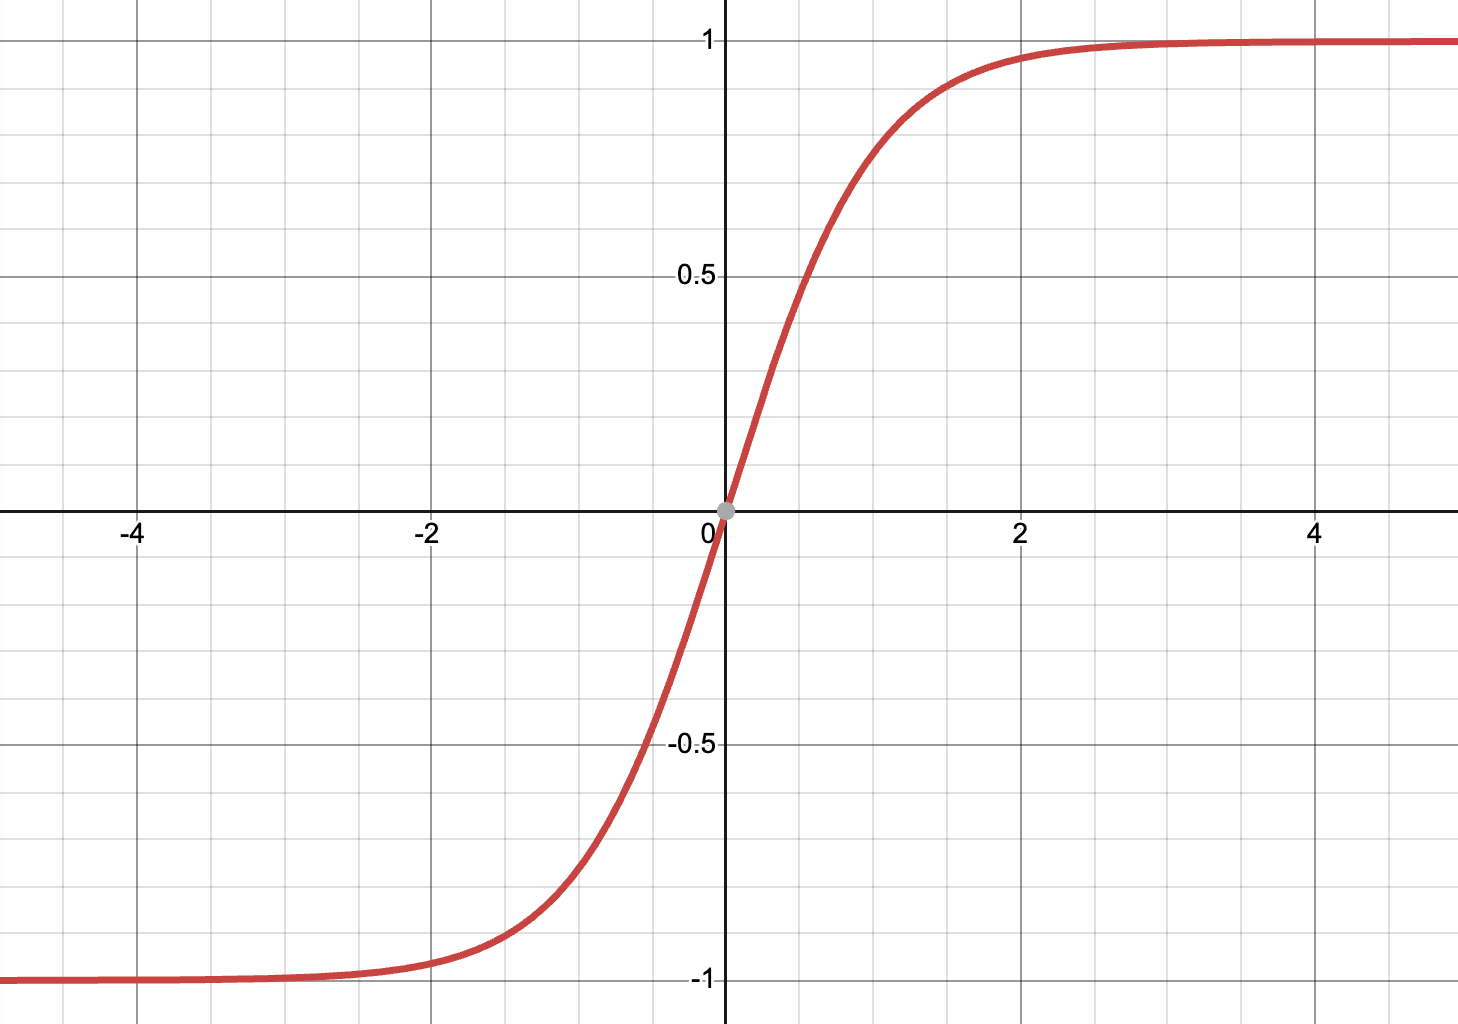
\includegraphics[width=\textwidth/2]{figures/2-sota/activation/tanh.png}
    \caption[Leaky Relu Activation Function]{Very similar to Relu but with non-zero gradient for negative inputs.}
    \label{fig:leaky-relu}
\end{figure}
\paragraph{Backpropagation Algorithm for Training Neural Networks} \label{sec:backpropagation}

\textit{Backpropagation} is an algorithm used to train feedforward neural networks by computing the gradient of the loss function concerning the network weights. This gradient is then used to update the weights in the opposite direction of the gradient, allowing the network to learn how to predict outputs given inputs accurately.

To understand backpropagation, it is crucial to define the loss function, which measures the network's performance on a given task. For instance, the cross-entropy loss is commonly used in classification tasks to quantify the difference between predicted probabilities and the correct labels. More information on loss functions can be found in Section \ref{sec:loss-functions}. Backpropagation adjusts the network weights to minimize the loss function.

The backpropagation algorithm works by computing the gradient of the loss function concerning each weight in the network. This gradient tells how much the loss function would change if one were to make a small change to the weight. This gradient is then used to update the weight in the direction that reduces the loss function.

The gradient is computed using the chain rule of calculus. Considering a simple feedforward neural network with one hidden layer. The output of the network is given by:

\begin{equation}
	y = h(\sum_{j=1}^M w_{2,j} h(\sum_{i=1}^N w_{1,i} x_i + b_1) + b_2)
\end{equation}

where $x_i$ is the $i$-th input, $w_{1, i}$ and $w_{2, j}$ are the weights connecting the input to the hidden layer and the hidden layer to the output, respectively, $b_1$ and $b_2$ are the biases of the hidden layer and the output, respectively, $h$ is the activation function, such as sigmoid, (see section \ref{sec:activation}), and $N$ and $M$ are the numbers of inputs and hidden units, respectively.

The loss function is a function of the output $y$ and the actual label $t$.

To compute the gradient of the loss function concerning a weight $w_{i,j}$, one first needs to compute the local gradient of the output for the weight. This is given by:

\begin{equation}
	\frac{\partial y}{\partial w_{i,j}} = h'(\sum_{j=1}^M w_{2,j} h(\sum_{i=1}^N w_{1,i} x_i + b_1) + b_2) h(\sum_{i=1}^N w_{1,i} x_i + b_1) w_{2,j}
\end{equation}

where $h'$ is the derivative of the activation function. One can then use the chain rule to compute the gradient of the loss function for the weight:

\begin{equation}
	\frac{\partial E}{\partial w_{i,j}} = (y - t)\frac{\partial y}{\partial w_{i,j}}
\end{equation}

Once one has computed the gradient of the loss function concerning all the weights in the network, the weights can be updated using gradient descent:

\begin{equation}
	w_{i,j} \leftarrow w_{i,j} - \alpha \frac{\partial E}{\partial w_{i,j}}
\end{equation}

where $\alpha$ is the learning rate, which determines the step size of the weight update.

Backpropagation can be extended to networks with multiple hidden layers using the chain rule to propagate the gradient backward through the network.
\paragraph{Optimization with Stochastic Gradient Descent} \label{sec:sgd}

\Acf{SGD} is a widely used optimization algorithm in \ac{DL}. It is an iterative method that minimizes the loss function by updating the model parameters in the direction of the negative gradient of the loss function. In each iteration, \ac{SGD} randomly selects a subset of the training data, called a mini-batch, and computes the gradient of the loss function concerning the parameters using the mini-batch. The parameters are then updated by subtracting the product of the gradient and a learning rate hyperparameter, which controls the step size of the update. The learning rate is typically set to a small value to ensure the stability and convergence of the algorithm.

Technically, it would be possible to use the loss of all the samples to update the model weights. However, using all the samples to update the weights, also known as batch gradient descent, can be computationally expensive and memory-intensive, especially for large datasets. In contrast, \ac{SGD} updates the weights based on a randomly selected sample mini-batch, reducing the computational and memory requirements and enabling faster convergence.

Moreover, \ac{SGD} introduces stochasticity in the optimization process, which can help the algorithm escape from local minima and explore different regions of the parameter space. This can improve the model's generalization performance and prevent overfitting the training data.

However, \ac{SGD} can also be noisier and less stable than batch gradient descent due to the mini-batches random sampling and the gradients' fluctuation. Therefore, finding an appropriate learning rate and mini-batch size is crucial for the solutions' convergence and quality in \ac{SGD}.

Formally, let $\theta$ be the vector of model parameters, $L(\theta)$ be the loss function, $D$ be the training dataset, and $B$ be a mini-batch sampled from $D$. Then, the update rule for \ac{SGD} can be written as:

\begin{equation}
	\theta_{t+1} = \theta_{t} - \alpha \nabla_{\theta} L(\theta_t; B)
\end{equation}

where $\alpha$ is the learning rate, and $\nabla_{\theta} L(\theta_t; B)$ is the gradient of the loss function concerning the parameters evaluated on the mini-batch $B$ at iteration $t$.

\ac{SGD} has several advantages, such as its simplicity and low memory requirements, which make it suitable for large-scale datasets and complex models. However, it also has some limitations, such as its sensitivity to the learning rate and the mini-batch size, which can affect the solutions' convergence and quality. Therefore, several variants of \ac{SGD}, such as Adagrad (that adapts the learning rate for each parameter based on its historical gradients, working well for sparse data) and Adam (explained in Section \ref{sec:adam}, adds a fraction of the previous update to the current update, and adapts the learning rate), have been proposed to address these issues and improve the algorithm's performance.
\paragraph{Optimization with the Adam Optimizer} \label{sec:adam}

Adam is a variant of \ac{SGD} (see Section \ref{sec:sgd}) that adapts the learning rate for each parameter based on the estimates of the first and second moments of the gradients \cite{kingma_adam_2017}.

Adam addresses some of the limitations of \ac{SGD}, such as the sensitivity to the learning rate and the mini-batch size, using a more sophisticated update rule incorporating information about the gradients and their history. Specifically, Adam computes a moving average of the gradients and their squares, which adjusts the updates' learning rate and momentum.

The estimates of the moments are computed as follows:

\begin{equation}
    m_t = \beta_1 m_{t-1} + (1-\beta_1)g_t
\end{equation}

\begin{equation}
    v_t = \beta_2 v_{t-1} + (1-\beta_2)g_t^2
\end{equation}

where $g_t$ is the gradient of the loss function with respect to the parameters at iteration $t$, $m_{t-1}$ and $v_{t-1}$ are the estimates of the moments at the previous iteration, and $\beta_1$ and $\beta_2$ are the decay rates for the moving averages of the gradients and their squares, respectively.

The update rule for Adam can then be written as follows:

\begin{equation}
    \theta_{t+1} = \theta_{t} - \frac{\alpha}{\sqrt{\hat{v}_t+\epsilon}}\hat{m}_t
\end{equation}

where $\theta_t$ is the vector of model parameters at iteration $t$, $\alpha$ is the learning rate, $\hat{m}_t$ and $\hat{v}_t$ are the biased estimates of the first and second moments of the gradients, respectively, and $\epsilon$ is a small constant to avoid division by zero.

The biased estimates of the moments are computed as follows:

\begin{equation}
    \hat{m}_t = \frac{m_t}{1-\beta_1^t}
\end{equation}

\begin{equation}
    \hat{v}_t = \frac{v_t}{1-\beta_2^t}
\end{equation}

where $t$ is the iteration number. The bias correction is necessary to account for the fact that the estimates are initialized at zero and may be biased towards zero in the early iterations.

By using the biased estimates of the moments, Adam can handle noisy or sparse gradients and converge faster than SGD on a wide range of optimization problems. However, the choice of the hyperparameters, such as the learning rate, the decay rates, and the epsilon value, can significantly affect the performance of Adam and should be carefully tuned for each problem.

Adam combines the benefits of both momentum and adaptive learning rates by using the moving average of the gradients to update the momentum and the moving average of the squared gradients to adapt the learning rate. Unlike \ac{SGD}, which uses a fixed learning rate for all parameters, Adam adapts the learning rate individually for each parameter based on the estimate of the second moment of the gradient. This can improve the solutions' convergence and quality, especially for problems with sparse or noisy gradients. Moreover, Adam can handle non-stationary objective functions and noisy gradients, which can be challenging for other optimization algorithms.

However, Adam also has some limitations, such as its sensitivity to the choice of hyperparameters and its tendency to overshoot the optimal solution. Therefore, tuning the hyperparameters carefully and monitoring the algorithm's convergence during training is important.